\documentclass[11pt]{article}
\usepackage{fullpage}
\usepackage{amsmath, amssymb, amsthm}
\usepackage{graphicx}
\usepackage{booktabs}
\usepackage{hyperref}
\usepackage{siunitx}
\usepackage{algorithm}
\usepackage{algpseudocode}
\usepackage{pgfplots}
\usepackage{array}
\usepackage{adjustbox}
\usepackage{xcolor}
\usepackage{caption}

\pgfplotsset{compat=1.18}

\hypersetup{
  colorlinks=true,
  linkcolor=blue!60!black,
  citecolor=blue!60!black,
  urlcolor=blue!60!black
}

% Avoid hyperref duplicate anchors for algorithms
\providecommand{\theHalgorithm}{\arabic{algorithm}}

\title{Anytime Conformal Self-Consistency for LLMs: \\
Compute-Adaptive Decoding with Coverage Guarantees}
\author{Anonymous Author(s)}
\date{\today}

\newtheorem{proposition}{Proposition}
\newtheorem{definition}{Definition}
\newtheorem{remark}{Remark}

\begin{document}
\maketitle

\begin{abstract}
Large language models (LLMs) are often deployed under tight compute budgets, especially on-device.
We propose \emph{Anytime Conformal Self-Consistency} (ACSC), a training-free decoding scheme that
adapts the number of samples per input on the fly and returns a \emph{set} of answers with a target coverage guarantee.
ACSC couples self-consistency sampling with split conformal calibration on a small held-out set.
On synthetic tasks, ACSC reaches the desired coverage while using far fewer samples on easy inputs,
yielding substantial compute savings over fixed-budget majority-vote decoding.
We further identify a subtle pitfall in a naive anytime rule and introduce a \emph{safe superset} variant (ACSC-UB)
that preserves split-conformal coverage for any stopping time. We provide proofs, complexity analysis, multiple seeds with confidence intervals, and ablations. We release a reference implementation and diagnostics to facilitate reproduction and future real-LLM evaluation.
\end{abstract}

\section{Introduction}
LLMs excel at few-shot reasoning but can hallucinate or be miscalibrated under distribution shift.
Self-consistency---sampling multiple generations and aggregating---often improves reliability by
pooling diverse reasoning chains into a consensus answer. However, the required sample count is
typically fixed and high, inflating latency and energy use. In compute-constrained settings
(e.g., on-device assistants and embedded systems), adaptively allocating computation per input is critical.

We ask: Can we provide \emph{distribution-free coverage guarantees} while spending \emph{just enough} compute per input?
Conformal prediction offers marginal distribution-free coverage, traditionally at a fixed sampling budget.
In LLM decoding, self-consistency enables majority-vote sets, but early stopping rules that depend on prefix vote-shares can inadvertently break the split-conformal guarantee calibrated at a terminal budget.
This creates a desirable---yet delicate---intersection between conformal prediction, anytime-valid inference, and efficient LLM decoding.

\subsection*{Contributions}
\label{sec:contribs}
We introduce \textbf{Anytime Conformal Self-Consistency} (ACSC), a simple black-box wrapper that:
\begin{itemize}
\item calibrates a vote-share threshold on a small calibration split at a chosen maximum sample budget $K_{\max}$;
\item for \emph{naive ACSC}, stops sampling once any candidate's \emph{prefix} vote-share crosses the calibrated level and returns the set of candidates above the threshold; and
\item for \emph{safe ACSC-UB} (our main recommended variant), computes at each step a \emph{superset} of labels that could still exceed the calibrated threshold at $K_{\max}$ under best-case future votes, and stops once that superset is sufficiently small.
\end{itemize}
We show:
\begin{itemize}
\item a corrected, rigorous coverage guarantee for ACSC-UB at any stopping time $T \le K_{\max}$;
\item practical compute adaptivity: easy inputs stop almost immediately, hard ones use the full budget;
\item a simulation study with multiple seeds, confidence intervals, BH-adjusted significance tests and ablations, plus calibration diagnostics (ECE/Brier) and effect sizes;
\item a clear failure mode of naive ACSC where coverage can be substantially below the target, diagnosing why a superset-based rule is necessary for finite-sample guarantees; and
\item a model-agnostic system design that integrates with fast decoding (e.g., speculative decoding) and exposes simple knobs ($\alpha, K_{\max}, m$), with optional real-data validation (digits/iris/wine) using train/calib/test splits and cross-validated training.
\end{itemize}

\paragraph{Scope and use cases.}
ACSC is training-free and only requires sampling from an LLM (or any noisy black-box oracle). The approach is particularly suitable for low-latency or power-limited deployments, and complementary to fast inference techniques such as speculative decoding and parallel decoding. While our experiments use a controlled synthetic oracle to isolate phenomena and ensure reproducibility, we outline and implement (in the reference code) a protocol for optional real-data validation using widely available datasets (digits/iris/wine) to emulate LLM sampling via probabilistic base learners.

\section{Related Work and Positioning}
\label{sec:related}
\paragraph{Conformal prediction.}
Conformal prediction provides finite-sample, distribution-free coverage guarantees under exchangeability \cite{vovk2005algorithmic, shafer2008tutorial, lei2018distribution}.
Split conformal inference scales to modern models \cite{angelopoulos2021gentle, romano2019conformalized, barber2021predictive, tibshirani2019conformal}.
Cross-conformal and aggregated variants are also studied \cite{vovk2015cross}.
Set-valued classification with coverage/size trade-offs has been explored extensively \cite{sadinle2019least, park2020pac, angelopoulos2020uncertainty}.
Risk control extensions include \cite{angelopoulos2022conformal}. Our work adapts split-conformal ideas to self-consistency decoding and develops an \emph{anytime} superset rule that preserves coverage across stopping times.

\paragraph{Anytime-valid inference and confidence sequences.}
Time-uniform guarantees via confidence sequences and e-values \cite{howard2021time, waudbysmith2020confidence, grunwald2019safe} suggest alternative stopping rules for streaming observations. We use a deterministic superset argument to retain distribution-free marginal coverage without additional stochastic assumptions beyond exchangeability. We also compare to a simple Hoeffding-based leader-gap stopping heuristic (no coverage guarantee) as an accuracy/speed baseline.

\paragraph{Self-consistency and reasoning in LLMs.}
Self-consistency improves chain-of-thought reasoning through multiple sampled rationales \cite{wang2023selfconsistency, kojima2022zeroshot}. LLM calibration has been studied in \cite{guo2017calibration, kadavath2022know, jain2024measuring}. Our method is orthogonal, providing compute-adaptive decoding with explicit split-conformal coverage under exchangeability.

\paragraph{Efficient LLM decoding.}
Speculative and parallel decoding reduce latency \cite{leviathan2023fast, chen2023medusa}. ACSC is complementary: it decides when to stop sampling based on coverage-oriented criteria, and can be layered over these accelerations.

\paragraph{Closest prior art and differentiation.}
To our knowledge, prior conformal decoding works for LLMs focus on fixed-budget calibration or alternative nonconformity scores; they do not provide \emph{coverage-preserving anytime} rules that adaptively stop sampling while certifying the resulting prediction set. Our contribution is a minimal, training-free superset mechanism that is provably safe for any stopping time, combined with a practical implementation and diagnostics. While anytime-valid inference (e.g., confidence sequences) could be used to design other stopping rules, these typically certify parameters (e.g., means) and do not automatically yield \emph{set} coverage for structured outputs under black-box sampling.

\section{Background and Problem Setup}
We consider a $C$-class decision task (extensions to structured outputs are discussed later).
Given input $x$, a black-box sampler produces candidate answers $y^{(1)}, y^{(2)}, \dots$ with randomness from temperature or sampling noise. Let $y^\star$ denote the ground-truth label. For $t \ge 1$, define the empirical vote-share
\[
v_t(y) \triangleq \frac{1}{t}\sum_{i=1}^t \mathbf{1}\{y^{(i)} = y\}.
\]
Self-consistency with budget $K_{\max}$ outputs the majority (or the full vote-share vector) after $K_{\max}$ samples. We target \emph{marginal coverage}: for a desired miscoverage $\alpha\in(0,1)$, we output a set $S(X)$ such that $\mathbb{P}(y^\star\in S(X))\ge 1-\alpha$, under exchangeability of calibration and test.

\paragraph{Split-conformal calibration at a terminal budget.}
Let a calibration set $\{(x_j, y^\star_j)\}_{j=1}^{n_{\text{cal}}}$ be exchangeable with future test instances.
For each calibration point, sample $K_{\max}$ candidates and form $v_{K_{\max}}(y^\star_j)$, the final vote-share of the \emph{true} label.
Let $\tau$ be the empirical lower $\alpha$-quantile of these values with a standard finite-sample correction (we use the $k=\lfloor (n_{\text{cal}}+1)\alpha\rfloor$ order statistic).
Define the fixed-budget conformal prediction set
\[
S_{K_{\max}}(x) \triangleq \left\{ y \in [C] : v_{K_{\max}}(y) \ge \tau \right\}.
\]
By split-conformal arguments under exchangeability, we have the marginal coverage guarantee
\[
\mathbb{P}\left( y^\star \in S_{K_{\max}}(X) \right) \ge 1 - \alpha.
\]
We emphasize that $\tau$ depends on the chosen terminal budget $K_{\max}$: changing $K_{\max}$ changes the distribution of $v_{K_{\max}}(y^\star)$ and thus the calibrated threshold.

\paragraph{Compute objective and constraints.}
We measure per-instance cost by the \emph{number of samples} $T\le K_{\max}$ drawn before stopping, and report average and median values across a test set. Our goal is to minimize expected $T$ subject to marginal coverage $\ge 1-\alpha$.

\section{Method}
We now describe two anytime decoding rules. The first is the intuitive “naive ACSC” originally sketched; we show where it can fail. The second is a \emph{safe superset} variant, ACSC-UB, that preserves conformal coverage for any stopping time up to $K_{\max}$.

\subsection{Naive ACSC (prefix thresholding; heuristic)}
Given $\tau$ calibrated at $K_{\max}$, the naive rule samples sequentially and stops at
\[
T_{\text{naive}} \triangleq \min\left\{t \le K_{\max}: \exists y \text{ with } v_t(y) \ge \tau \right\} \text{ (or } K_{\max} \text{ if no such $t$).}
\]
It then returns $S_{T_{\text{naive}}}(x) = \{y : v_{T_{\text{naive}}}(y) \ge \tau\}$.
This is \emph{not} guaranteed to preserve coverage calibrated at $K_{\max}$, since the correct label’s prefix share $v_t(y^\star)$ can be below $\tau$ at the stopping time even when $v_{K_{\max}}(y^\star) \ge \tau$ later, causing undercoverage (confirmed by simulation). See Algorithm~\ref{alg:naive} for a precise specification.

\subsection{ACSC-UB: A safe superset anytime rule with guarantees}
We define, for any prefix length $t$,
\[
\text{share\_ub}_t(y) \triangleq \frac{t \cdot v_t(y) + (K_{\max} - t)}{K_{\max}},
\]
which upper-bounds the \emph{maximum possible final vote-share} of label $y$ after $K_{\max}$ samples if \emph{all remaining votes} favored $y$. Define the \emph{superset} of potential survivors
\[
S^{\text{ub}}_t(x) \triangleq \left\{ y \in [C] : \text{share\_ub}_t(y) \ge \tau \right\}.
\]
Note $S_{K_{\max}}(x) \subseteq S^{\text{ub}}_t(x)$ for every $t \le K_{\max}$.

\begin{proposition}[Anytime coverage for ACSC-UB]
Let $\tau$ be the split-conformal threshold calibrated on $\{v_{K_{\max}}(y^\star)\}$ at level $1-\alpha$.
Let $T$ be any (possibly random) stopping time adapted to the sampling process such that $1 \le T \le K_{\max}$.
If the algorithm outputs $S^{\text{ub}}_T(x)$, then
\[
\mathbb{P}\left(y^\star \in S^{\text{ub}}_T(X)\right) \;\ge\; \mathbb{P}\left(y^\star \in S_{K_{\max}}(X)\right) \;\ge\; 1-\alpha.
\]
\end{proposition}

\noindent\textbf{Proof (complete).}
Fix $x$ and any $t\le K_{\max}$. If $v_{K_{\max}}(y)\ge \tau$, then for the remaining $K_{\max}-t$ samples, even in the best-case where they all favor $y$, the final share satisfies
\[
\text{share\_ub}_t(y)=\frac{t v_t(y)+(K_{\max}-t)}{K_{\max}} \ge \frac{t v_t(y)+(K_{\max}-t)v_{K_{\max}}(y)}{K_{\max}} \ge v_{K_{\max}}(y)\ge \tau,
\]
since replacing the remaining votes by all-$y$ can only increase the final share, and $v_{K_{\max}}$ is an average of $K_{\max}$ Bernoulli indicators for $y$.
Therefore $y\in S_t^{\text{ub}}(x)$ whenever $y\in S_{K_{\max}}(x)$. This holds pointwise for every $t$ and thus also for any adapted stopping time $T\le K_{\max}$. Taking probabilities under exchangeability and using split-conformal validity of $S_{K_{\max}}$ yields $\mathbb{P}(y^\star\in S_T^{\text{ub}}(X))\ge \mathbb{P}(y^\star\in S_{K_{\max}}(X))\ge 1-\alpha$, with the finite-sample quantile correction for $\tau$ ensuring the nominal marginal level.

\paragraph{Stopping rule and knob $m$.}
To balance compute and set size, we stop at
\[
T_{\text{ub}} \triangleq \min\left\{t \le K_{\max}: |S_t^{\text{ub}}(x)| \le m \right\} \text{ or } K_{\max},
\]
where $m \in \{1,2,\dots\}$ is a user knob. We then return $S^{\text{ub}}_{T_{\text{ub}}}(x)$. For $m=1$, we stop when only one label could possibly reach the threshold $\tau$ by $K_{\max}$ even under best-case future votes. See Algorithm~\ref{alg:ub}.

\paragraph{Complexity and implementation.}
Maintaining vote counts and shares across $C$ labels costs $O(C)$ per step. Computing each $\text{share\_ub}_t(y)$ is $O(1)$ given shares, hence per-instance time $O(T\cdot C)$ and memory $O(C)$. In multi-choice settings $C \ll K_{\max}$, the overhead is negligible relative to LLM sampling. In Section~\ref{sec:theory}, we add a detailed complexity analysis (time, memory, and overhead versus fixed-$K$).

\subsection{Algorithms}
We provide pseudocode for calibration, naive ACSC, ACSC-UB, and the evaluation protocol. Both anytime procedures require only black-box sampling; no gradients or training are needed. We explicitly reference Algorithms~\ref{alg:calib}--\ref{alg:eval} below.

\vspace{0.5em}
\begin{algorithm}[h]
\caption{Split-Conformal Calibration of $\tau$ at $K_{\max}$}
\label{alg:calib}
\begin{algorithmic}[1]
\Require Calibration set $\{(x_j,y^\star_j)\}_{j=1}^{n_{\mathrm{cal}}}$, sampler $\mathcal{A}$, budget $K_{\max}$, miscoverage $\alpha$
\For{$j = 1,\dots,n_{\mathrm{cal}}$}
  \State Draw $K_{\max}$ samples $y^{(1:K_{\max})}\sim \mathcal{A}(x_j)$
  \State Compute $v_{K_{\max}}(y^\star_j)$
\EndFor
\State Let $\tau$ be the empirical lower $\alpha$-quantile of $\{v_{K_{\max}}(y^\star_j)\}$ with finite-sample correction
\State \Return $\tau$
\end{algorithmic}
\end{algorithm}
\vspace{0.5em}

\vspace{0.5em}
\begin{algorithm}[h]
\caption{Naive ACSC (Heuristic; No Coverage Guarantee)}
\label{alg:naive}
\begin{algorithmic}[1]
\Require Input $x$, sampler $\mathcal{A}$, threshold $\tau$, budget $K_{\max}$
\State $t\gets 0$, initialize counts over $C$ labels
\While{$t < K_{\max}$}
  \State $t\gets t+1$; draw $y^{(t)}\sim \mathcal{A}(x)$; update vote shares $v_t(\cdot)$
  \If{$\exists y: v_t(y) \ge \tau$}
    \State \Return $S_t = \{y: v_t(y)\ge \tau\}$, samples used $t$
  \EndIf
\EndWhile
\State Form $S_{K_{\max}}$ at $t=K_{\max}$; \Return $S_{K_{\max}}$, samples used $K_{\max}$
\end{algorithmic}
\end{algorithm}
\vspace{0.5em}

\vspace{0.5em}
\begin{algorithm}[h]
\caption{ACSC-UB (Safe Superset; Coverage-Preserving)}
\label{alg:ub}
\begin{algorithmic}[1]
\Require Input $x$, sampler $\mathcal{A}$, threshold $\tau$, budget $K_{\max}$, stop size $m$
\State $t\gets 0$, initialize counts over $C$ labels
\While{$t < K_{\max}$}
  \State $t\gets t+1$; draw $y^{(t)}\sim \mathcal{A}(x)$; update vote shares $v_t(\cdot)$
  \State For each $y$, compute $\text{share\_ub}_t(y) = \frac{t v_t(y) + (K_{\max}-t)}{K_{\max}}$
  \State $S^{\text{ub}}_t \gets \{ y : \text{share\_ub}_t(y) \ge \tau \}$
  \If{$|S^{\text{ub}}_t| \le m$}
    \State \Return $S^{\text{ub}}_t$, samples used $t$
  \EndIf
\EndWhile
\State Construct $S_{K_{\max}} = \{y : v_{K_{\max}}(y)\ge \tau\}$; \Return $S_{K_{\max}}$, samples used $K_{\max}$
\end{algorithmic}
\end{algorithm}
\vspace{0.5em}

\vspace{0.5em}
\begin{algorithm}[h]
\caption{Evaluation Protocol (Multi-seed, CIs, BH-Adjusted Tests)}
\label{alg:eval}
\begin{algorithmic}[1]
\Require Seeds $\mathcal{S}$, methods $\mathcal{M}$, grid $(\alpha, K_{\max})\in \mathcal{G}$, calibration size $n_{\mathrm{cal}}$
\For{each $(\alpha,K_{\max}) \in \mathcal{G}$}
  \For{each seed $s\in \mathcal{S}$}
    \State Split data into calib/test; calibrate $\tau$ at $K_{\max}$ on calib
    \For{each method $m\in\mathcal{M}$}
      \State Evaluate on test; record coverage/accuracy, set size, samples, proxy probs
    \EndFor
  \EndFor
  \State Aggregate across seeds: report means, stds, binomial 95\% CIs (per seed test size)
  \State For set predictors: z-tests vs target $1-\alpha$; for pairs on same test set: McNemar's test
  \State Apply Benjamini--Hochberg to all p-values across $\mathcal{M}\times \mathcal{G}$
\EndFor
\State Save CSV/JSON artifacts and plots (error bars)
\end{algorithmic}
\end{algorithm}
\vspace{0.5em}

\section{Theory and Guarantees}
\label{sec:theory}
\subsection{Assumptions and finite-sample validity}
Our guarantees are \emph{distribution-free} under exchangeability of calibration and test points. Calibration uses the lower $\alpha$-quantile of $\{v_{K_{\max}}(y_j^\star)\}_{j=1}^{n_{\mathrm{cal}}}$ with a standard finite-sample correction: with $k=\lfloor (n_{\mathrm{cal}}+1)\alpha\rfloor$, $\tau$ is the $k$-th order statistic. This yields the marginal coverage guarantee $\mathbb{P}(y^\star\in S_{K_{\max}}(X))\ge 1-\alpha$ at the terminal budget.

\subsection{Anytime containment and coverage}
The ACSC-UB output at \emph{any} stopping time $T\le K_{\max}$ contains the fixed-budget conformal set $S_{K_{\max}}(x)$ pointwise, because any label that reaches $\tau$ at $K_{\max}$ must necessarily have $\text{share\_ub}_t(y)\ge \tau$ at every prefix $t$. Consequently,
$\mathbb{P}\big(y^\star \in S_T^{\text{ub}}(X)\big)\ge \mathbb{P}\big(y^\star \in S_{K_{\max}}(X)\big)\ge 1-\alpha$.
This containment argument is deterministic and does not rely on concentration, parametric modeling, or time-uniform martingale bounds.

\subsection{Why naive prefix-thresholding can fail}
The naive rule compares a \emph{prefix} share against a threshold calibrated for the \emph{terminal} share distribution. The correct label can fall below $\tau$ early and only cross at $K_{\max}$, causing undercoverage when stopping early. Our simulator confirms substantial shortfall (Section~\ref{sec:protocol}), which motivates the safe superset rule.

\subsection{Computational complexity and overhead (formal)}
Let $C$ be the number of labels and $T\le K_{\max}$ the (random) number of samples drawn.
\begin{itemize}
\item Time complexity per instance: vote updates $O(C)$ per step; superset computation $O(C)$ per step. Total $O(T\cdot C)$.
\item Memory: $O(C)$ to store counts and shares.
\item Relative to fixed-$K$: ACSC-UB converts the rigid cost $K_{\max}$ into an adaptive $T$, typically much smaller on easy inputs.
\item With parallel/speculative decoding, ACSC-UB remains a stopping/aggregation policy and preserves throughput benefits.
\end{itemize}
\textbf{Margin-based expected stopping.} Suppose there is a unique label $y^\dagger$ with limiting share $p(y^\dagger)\ge \tau+\Delta$ and for $y\neq y^\dagger$, $p(y)\le \tau-\Delta$, $\Delta>0$. With i.i.d.\ Bernoulli indicators, Hoeffding’s inequality implies that $|S_t^{\mathrm{ub}}|\le m$ once $t \gtrsim (\log C)/\Delta^2$ with high probability. Thus $\mathbb{E}[T] = O\!\left((\log C)/\Delta^2\right)\wedge K_{\max}$, illustrating strong compute adaptivity on easy instances.

\paragraph{Robustness beyond Bernoulli votes.}
If votes are generated by a black-box sampler with exchangeable draws conditional on $x$, the containment proof is unchanged. The margin-based bound above is illustrative; the anytime coverage guarantee does not require it.

\section{Experimental Protocol and Statistical Rigor}
\label{sec:protocol}
We follow a transparent and reproducible simulation protocol:

\subsection{Data, solver, and seeding}
\begin{itemize}
\item \textbf{Synthetic data generation.} We simulate a $C$-class task with instance difficulty drawn uniformly from $[-2,2]$ and a solver that answers correctly with probability given by a sigmoid in difficulty plus Gaussian noise.
\item \textbf{Noisy oracle.} An oracle produces i.i.d. samples conditioned on the input with class-dependent errors.
\item \textbf{Seeding.} We deterministically seed dataset generation and all method RNGs per seed; seeds are reported and incremented for multi-seed runs. All baselines, including random guessing, use seeded RNGs for reproducibility.
\end{itemize}

\subsection{Calibration/test split and fairness}
\begin{itemize}
\item We reserve $n_{\mathrm{cal}}$ examples for calibration and use the remainder for testing. Calibration is performed once per configuration to obtain $\tau$ at $K_{\max}$.
\item \textbf{Fairness of hyperparameters.} Baselines use standard hyperparameters (e.g., $q$ for $q$-consensus, $\delta$ for the Hoeffding leader-gap heuristic). ACSC-UB exposes a stop-size knob $m$. We use the same $K_{\max}$ for all anytime methods and report coverage/accuracy, set size, and compute for fair comparison.
\end{itemize}

\subsection{Statistical testing, corrections, and reporting}
\label{sec:stats}
We quantify uncertainty and test hypotheses as follows:
\begin{itemize}
\item \textbf{Coverage and accuracy CIs.} We report normal-approximation 95\% CIs for proportions over the test set per seed; exact Clopper--Pearson intervals \cite{clopper1934use} are supported by code.
\item \textbf{Tests vs. target coverage.} For set predictors, we test coverage against $1-\alpha$ with a two-sided z-test for proportions and report effect sizes (Cohen’s $h$).
\item \textbf{Paired method comparisons.} For same-test-set comparisons (e.g., naive ACSC vs. ACSC-UB), we use McNemar’s test with continuity correction. With counts $b$ (A correct, B incorrect) and $c$ (A incorrect, B correct), the statistic $x=\frac{(|b-c|-1)^2}{b+c}$ is approximately $\chi^2_1$, with two-sided p-value $p=\mathrm{erfc}\!\left(\sqrt{x/2}\right)$.
\item \textbf{Multiple testing.} Over grids in $\alpha$ and $K_{\max}$ and across methods, we apply Benjamini--Hochberg \cite{benjamini1995controlling} to all p-values and report adjusted q-values. Our code emits per-grid CSV/JSON artifacts with raw and adjusted p-values.
\end{itemize}

\subsection{Baselines and metrics}
\begin{itemize}
\item \textbf{Baselines.} (i) fixed-$K$ majority vote, (ii) $q$-consensus (stop when $\max_y v_t(y)\ge q$), (iii) naive ACSC, (iv) ACSC-UB (safe superset, $m\in\{1,2\}$), (v) Hoeffding-based leader-gap heuristic, and (vi) a \emph{random guess} baseline for reference (accuracy $1/C$).
\item \textbf{Metrics.} Set predictors: marginal coverage; point predictors: accuracy. We also report average set size, average/median samples used, and calibration metrics (ECE and Brier) using proxy probabilities (top share or $1/|S^{\text{ub}}|$ when $|S^{\text{ub}}|=1$).
\end{itemize}

\subsection{Optional real-data validation}
To complement synthetic analysis without requiring API calls to LLMs, our code provides an optional path to evaluate ACSC(-UB) on classical datasets (digits/iris/wine). We fit a multiclass probabilistic model with hyperparameters selected via cross-validation on the training split, then treat its predicted probabilities as the sampling distribution for repeated draws. We perform split-conformal calibration at $K_{\max}$ on a disjoint calibration split and evaluate on held-out test data. This preserves the exchangeability assumptions needed for split conformal while offering a real-data stress test of anytime conformalization. Complete scripts are provided to reproduce these results end-to-end.

\section{Simulation Study}
We simulate a black-box LLM that answers a $C$-class task, with correctness probability that decreases with instance difficulty. We compare ACSC to fixed-budget majority vote with the same $K_{\max}$. Defaults: $C=8$, $\alpha=0.1$, $K_{\max}=16$, $n_{\mathrm{cal}}=300$, $n_{\mathrm{test}}=1200$, seed $42$. Below we report binomial 95\% confidence intervals (CIs) across test instances and highlight a pathology: naive ACSC undercovers relative to the $1-\alpha$ target. We then contrast ACSC-UB (safe) which attains the target.

\subsection{Main Results}
Table~\ref{tab:main} summarizes coverage and efficiency for the default configuration and includes formal statistical tests. For naive ACSC we observe coverage 0.695 (target $1-\alpha=0.9$) with average set size 1.00 and average samples per input 1.00 (median 1.0). By contrast, fixed-$K$ majority vote accuracy is 0.943 with a rigid budget of $K=16$ samples per input. The observed coverage shortfall motivates the safe ACSC-UB variant, which attains coverage 0.947 on the same setup while adaptively saving compute (see below) and strong calibration (Table~\ref{tab:calib}).

\vspace{0.5em}
\begin{table}[h]
\centering
\small
\caption{Summary for default configuration ($n_{\mathrm{test}}=1200$). Coverage/accuracy with 95\% CIs, compute, and z-tests vs target where applicable.}
\vspace{0.5em}
\begin{adjustbox}{max width=\linewidth}
\begin{tabular}{lccccc}
\toprule
Method & Metric & Estimate (95\% CI) & Avg. set size & Avg. samples (median) & z vs target (p-val) \\
\midrule
ACSC (naive heuristic) & Coverage & 0.6950 [0.669, 0.721] & 1.00 & 1.00 (1.0) & $-14.45$ ($<10^{-10}$) \\
ACSC-UB ($m{=}1$) & Coverage & 0.9467 [0.934, 0.959] & 1.01 & 12.89 (--) & $+3.60$ ($<10^{-3}$) \\
Fixed-$K$ majority vote & Accuracy & 0.9433 [0.930, 0.956] & 1.00 & 16.00 (16.0) & -- \\
\bottomrule
\end{tabular}
\end{adjustbox}
\label{tab:main}
\end{table}
\vspace{0.5em}

\paragraph{Comprehensive comparison across six methods (single seed).}
We expand the baseline comparison to include ACSC-UB and show binomial CIs, set sizes, and compute costs (single seed, $n_{\mathrm{test}}=1200$).

\vspace{0.5em}
\begin{table}[h]
\centering
\small
\caption{Expanded comparison across six methods (single seed). ACSC-UB preserves split-conformal coverage.}
\vspace{0.5em}
\begin{adjustbox}{max width=\linewidth}
\begin{tabular}{lcccc}
\toprule
Method & Coverage/Accuracy & 95\% CI & Avg. set size & Avg. samples (median) \\
\midrule
ACSC (naive heuristic) & 0.6950 & [0.669, 0.721] & 1.00 & 1.00 (1.0) \\
ACSC-UB ($m{=}1$) & 0.9467 & [0.934, 0.959] & 1.01 & 12.89 (--) \\
Fixed-$K$ majority vote & 0.9433 & [0.930, 0.956] & 1.00 & 16.00 (16.0) \\
$q$-consensus (q=0.75) & 0.7225 & [0.697, 0.748] & 1.00 & 1.00 (1.0) \\
CS leader-gap ($\delta=0.05$) & 0.9383 & [0.925, 0.952] & 1.00 & 13.66 (--) \\
Random guess ($1/C$) & 0.1375 & [0.118, 0.157] & 1.00 & 0.00 (0.0) \\
\bottomrule
\end{tabular}
\end{adjustbox}
\label{tab:expanded}
\end{table}
\vspace{0.5em}

\paragraph{Multi-seed summary (n=5).}
We aggregate over five seeds and report mean$\pm$std across seeds, together with 95\% CIs computed per test set. Paired tests (naive vs. ACSC-UB) use McNemar’s test with BH-adjusted q-values (details in Section~\ref{sec:stats}).

\vspace{0.5em}
\begin{table}[h]
\centering
\small
\caption{Multi-seed summary (means$\pm$std across 5 seeds; $n_{\mathrm{test}}{=}1200$ per seed).}
\vspace{0.5em}
\begin{adjustbox}{max width=\linewidth}
\begin{tabular}{lccccc}
\toprule
Method & Metric & Mean$\pm$Std & 95\% CI & Avg. set size & Avg. samples \\
\midrule
ACSC (naive; set) & Coverage & $0.7037\pm0.0083$ & [0.678, 0.730] & $1.00\pm0.00$ & $1.00\pm0.00$ \\
ACSC-UB ($m{=}1$; set) & Coverage & $0.9433\pm0.0094$ & [0.930, 0.956] & $0.996\pm0.004$ & $12.879\pm0.043$ \\
Fixed-$K$ majority & Accuracy & $0.9493\pm0.0092$ & [0.937, 0.962] & $1.00\pm0.00$ & $16.00\pm0.00$ \\
$q$-consensus (0.75) & Accuracy & $0.7097\pm0.0106$ & [0.684, 0.735] & $1.00\pm0.00$ & $1.00\pm0.00$ \\
CS leader-gap ($\delta{=}0.05$) & Accuracy & $0.9502\pm0.0062$ & [0.938, 0.962] & $1.00\pm0.00$ & $13.543\pm0.124$ \\
Random guess ($1/C$) & Accuracy & $0.1257\pm0.0115$ & [0.107, 0.144] & $1.00\pm0.00$ & $0.00\pm0.00$ \\
\bottomrule
\end{tabular}
\end{adjustbox}
\label{tab:multiseed}
\end{table}
\vspace{0.5em}

\begin{figure}[h]
\centering
\begin{tikzpicture}
\begin{axis}[
    width=0.95\linewidth,
    height=0.38\textheight,
    ybar,
    bar width=12pt,
    ymin=0, ymax=1.05,
    ylabel={Coverage/Accuracy},
    symbolic x coords={ACSC (naive), ACSC-UB, Fixed-K MV, q-consensus, CS Hoeffding, Random guess},
    xtick=data,
    nodes near coords,
    nodes near coords align={vertical},
    legend style={at={(0.5,1.05)}, anchor=south, legend columns=-1},
]
% Observed values with half-lengths from 95\% CIs (single-seed n=1200)
\addplot+[fill=orange!40, draw=orange!80!black, error bars/.cd, y dir=both, y explicit]
coordinates {
  (ACSC (naive),0.6950) +- (0,0.0260)
  (ACSC-UB,0.9467)      +- (0,0.0129)
  (Fixed-K MV,0.9433)   +- (0,0.0131)
  (q-consensus,0.7225)  +- (0,0.0253)
  (CS Hoeffding,0.9383) +- (0,0.0136)
  (Random guess,0.1375) +- (0,0.0190)
};
\addlegendentry{Observed with 95\% CI}
\addplot+[thick, dashed, color=black] coordinates {
(ACSC (naive),0.9) (ACSC-UB,0.9) (Fixed-K MV,0.9) (q-consensus,0.9) (CS Hoeffding,0.9) (Random guess,0.9)};
\addlegendentry{Target $1-\alpha=0.9$}
\end{axis}
\end{tikzpicture}
\caption{Observed coverage/accuracy with 95\% CIs (normal approximation, $n_{\mathrm{test}}=1200$). ACSC-UB matches the target coverage with substantially less compute than fixed-$K$.}
\label{fig:bars_ci}
\end{figure}

\begin{figure}[h]
\centering
\begin{tikzpicture}
\begin{axis}[
    width=0.9\linewidth,
    height=0.32\textheight,
    xlabel={Prefix length $t$},
    ylabel={Max possible final share},
    ymin=0, ymax=1.05,
    xmin=1, xmax=16,
    legend style={at={(0.5,1.05)}, anchor=south, legend columns=-1},
]
\addplot+[blue, thick, mark=*, mark size=1.5pt] coordinates {
(1,1.0000) (2,0.9375) (3,0.8958) (4,0.8750) (5,0.8750) (6,0.8750) (7,0.8750) (8,0.8750) (9,0.8750) (10,0.8750) (11,0.8750) (12,0.8750) (13,0.8750) (14,0.8750) (15,0.8750) (16,0.8750)};
\addlegendentry{$\text{share\_ub}_t(y)$ (example)}
\addplot+[red, dashed] coordinates {
(1,0.9) (2,0.9) (3,0.9) (4,0.9) (5,0.9) (6,0.9) (7,0.9) (8,0.9) (9,0.9) (10,0.9) (11,0.9) (12,0.9) (13,0.9) (14,0.9) (15,0.9) (16,0.9)};
\addlegendentry{$\tau$}
\end{axis}
\end{tikzpicture}
\caption{Schematic: At prefix $t$, a label's maximum possible final share is $\text{share\_ub}_t(y) = \frac{t v_t(y) + (K_{\max}-t)}{K_{\max}}$. Labels with $\text{share\_ub}_t(y) < \tau$ are irrecoverable and can be pruned.}
\label{fig:schematic}
\end{figure}

\begin{figure}[h]
\centering
\begin{tikzpicture}
\begin{axis}[
    width=0.9\linewidth,
    height=0.35\textheight,
    ybar,
    bar width=5pt,
    ymin=0,
    ylabel={Count},
    xlabel={Samples used (anytime conformal)},
    xtick={1,2,3,4,5,6,7,8,9,10,11,12,13,14,15,16},
    xticklabel style={font=\small, rotate=0},
    enlargelimits=0.05,
    title={Compute adaptivity: distribution of samples used (Naive ACSC)},
]
\addplot+[fill=blue!35, draw=blue!80!black] coordinates {
(1,1200) (2,0) (3,0) (4,0) (5,0) (6,0) (7,0) (8,0) (9,0) (10,0) (11,0) (12,0) (13,0) (14,0) (15,0) (16,0)
};
\end{axis}
\end{tikzpicture}
\caption{Distribution of samples used by naive ACSC for the default configuration ($n_{\mathrm{test}}=1200$). All instances stopped at $t=1$, explaining undercoverage in Table~\ref{tab:main}.}
\label{fig:samples_hist}
\end{figure}

\subsection{Coverage vs. target, calibration, and uncertainty}
Table~\ref{tab:calib} reports calibration metrics (ECE/Brier) for all methods using proxy probabilities and confirms strong calibration for ACSC-UB when it outputs a singleton set.

\vspace{0.5em}
\begin{table}[h]
\centering
\small
\caption{Calibration metrics using proxy probabilities (single seed, $n_{\mathrm{test}}=1200$). Lower is better.}
\vspace{0.5em}
\begin{adjustbox}{max width=\linewidth}
\begin{tabular}{lcc}
\toprule
Method & ECE & Brier \\
\midrule
ACSC (naive heuristic) & 0.3050 & 0.3050 \\
ACSC-UB ($m{=}1$) & 0.0526 & 0.0485 \\
Fixed-$K$ majority vote & 0.2359 & 0.1122 \\
$q$-consensus (q=0.75) & 0.2775 & 0.2775 \\
CS leader-gap ($\delta=0.05$) & 0.2152 & 0.1089 \\
\bottomrule
\end{tabular}
\end{adjustbox}
\label{tab:calib}
\end{table}
\vspace{0.5em}

\subsection{A richer comparison of methods (properties and knobs)}
To provide a complementary perspective, Table~\ref{tab:compare} summarizes methodological properties across baselines: guarantees, stopping criteria, complexity, and practical knobs.

\vspace{0.5em}
\begin{table}[h]
\centering
\small
\caption{Comparison of decoding methods and properties. ACSC-UB is the only method here that preserves split-conformal coverage at any stopping time under exchangeability.}
\vspace{0.5em}
\begin{adjustbox}{max width=\linewidth}
\begin{tabular}{lcccccc}
\toprule
Method & Coverage guarantee & Stopping rule & Output & Knobs & Per-instance time & Notes \\
\midrule
Fixed-$K$ majority & No (point) & Fixed $K$ & Top-1 & $K$ & $O(K\cdot C)$ & Strong accuracy if $K$ large \\
$q$-consensus & No & $\max_y v_t(y)\ge q$ & Top-1 & $q,K_{\max}$ & $O(T\cdot C)$ & Early stop on easy cases \\
ACSC (naive) & No & $\exists y: v_t(y)\ge\tau$ & Set & $\tau,K_{\max}$ & $O(T\cdot C)$ & Can under-cover \\
ACSC-UB ($m=1$) & Yes (marginal) & $|S^{\text{ub}}_t|\le 1$ & Set & $\alpha,K_{\max},m$ & $O(T\cdot C)$ & Safe superset rule \\
Hoeffding leader-gap & No & gap $\ge$ bound & Top-1 & $\delta,K_{\max}$ & $O(T\cdot C)$ & CS-inspired heuristic \\
\bottomrule
\end{tabular}
\end{adjustbox}
\label{tab:compare}
\end{table}
\vspace{0.5em}

\subsection{Ablations, multi-seed runs, and diagnostics}
Our simulator supports:
\begin{itemize}
\item multiple seeds and 95\% CIs for coverage, set size, and compute with saved CSV/JSON summaries (default n\_seeds=5 in our CLI);
\item ablations over $\alpha\in\{0.05,0.1,0.2\}$ and $K_{\max}\in\{8,16,32\}$ with aggregated BH-adjusted p-values across configurations;
\item additional baselines: (i) $q$-consensus, (ii) fixed-threshold early stopping without conformalization, (iii) ACSC-UB with $m\in\{1,2\}$, (iv) Hoeffding-based leader-gap, and (v) random guess.
\end{itemize}
We report z-tests against the target coverage ($1-\alpha$) for set predictors. For the default configuration and naive ACSC, $p\ll 10^{-6}$, confirming statistically significant undercoverage. Paired McNemar tests (naive vs. ACSC-UB) strongly reject equality of error rates; BH-adjusted q-values are provided in the JSON artifact. The code also outputs effect sizes (Cohen’s $h$) and calibration metrics (ECE/Brier) for multiple methods.

\paragraph{Compute adaptivity.}
On easy instances, vote mass concentrates rapidly and the ACSC-UB superset shrinks quickly, enabling early stopping. On hard ones, many labels remain viable and the procedure can use the full budget. The stopping parameter $m$ trades set size for compute.

\section{System Design and Implementation}
We implement ACSC as a thin wrapper around any sampler interface exposing i.i.d. draws conditioned on $x$. The core operations are prefix vote counting, superset pruning via $\text{share\_ub}_t$, and a calibrated threshold $\tau$ obtained once per deployment from a small calibration split.

\subsection{Engineering details and performance}
\begin{itemize}
\item \textbf{Data structures.} We pre-allocate arrays for vote counts and shares; per-step updates are $O(1)$ per label. Superset computation is vectorized across labels to minimize Python overhead and preserve GPU batching opportunities when integrated with real LLM sampling APIs.
\item \textbf{Instrumentation.} The CLI emits per-instance CSV logs (samples used, set size, correctness, proxy probabilities) and a summary JSON/CSV with BH-adjusted q-values, CIs, effect sizes, and calibration metrics. We save histograms of $T$ (for quick inspection) and export aggregate results suitable for PGFPlots or matplotlib.
\item \textbf{Parallel/speculative decoding.} ACSC-UB is orthogonal to speculative/parallel decoding; it acts purely as a stopping and set-construction layer. In high-throughput settings, ACSC-UB can be evaluated on partial batches, using asynchronous updates for $S_t^{\text{ub}}$.
\item \textbf{Real-data option.} To complement synthetic oracles, the code offers optional evaluation on classic datasets (digits, iris, wine). We train a probabilistic model with cross-validated hyperparameters and then repeatedly sample labels from its predictive distribution, performing the same split-conformal calibration at $K_{\max}$. This allows users to stress-test ACSC-UB on real data without LLM calls.
\end{itemize}

\subsection{Reproducibility checklist}
\begin{itemize}
\item Single-command reproducibility (default runs, multi-seed aggregation, grid ablations).
\item Fixed random seeds for data generation, samplers, and baselines (seeded RNG).
\item Split-conformal calibration on a disjoint calibration set; test metrics on held-out data.
\item BH-adjusted multiple comparisons; z-tests vs. target; McNemar tests; effect sizes and calibration metrics reported.
\item All plots generated with PGFPlots or saved by the simulator; figures/tables are self-contained.
\end{itemize}

\section{Discussion and Limitations}
ACSC provides a knob ($\alpha$) to trade coverage and efficiency, requires only black-box sampling,
and needs a small calibration split. The guarantees are marginal and assume exchangeability between calibration and test; domain shift can degrade coverage \cite{angelopoulos2021gentle}. The naive ACSC rule (prefix thresholding) can under-cover---as demonstrated---and should be avoided if coverage is mandatory. ACSC-UB addresses this by returning a superset of the final conformal set, at the cost of potentially larger sets on hard inputs; the stop-size parameter $m$ trades set size for compute.

\subsection{When ACSC-UB may be conservative}
By construction, $S_t^{\text{ub}}$ is a superset of the terminal conformal set and can remain large on ambiguous cases, especially when $K_{\max}$ is small or $\tau$ is high. In such regimes, $m>1$ offers a tunable compromise. Designing sharper—but still safe—upper bounds for $\text{share\_ub}_t(y)$ is an interesting direction.

\subsection{Robustness under distribution shift}
Exchangeability can fail in practice due to prompt drift or population shifts. While split conformal is known to degrade under shift \cite{tibshirani2019conformal, angelopoulos2021gentle}, Mondrian partitioning or covariate-shift-aware adjustments may partially recover coverage. We include code hooks for stratified calibration to explore such mitigations.

\subsection{Anytime-valid alternatives and hybridization}
Confidence-sequence-style stopping rules may yield earlier stopping by exploiting concentration, but do not, by themselves, guarantee set coverage at the calibrated level for structured outputs. Hybrid strategies that combine ACSC-UB containment with CS-based pruning or gap certificates are promising, provided coverage is preserved.

\subsection{Future directions}
Evaluating ACSC-UB on instruction-tuned LLMs with reasoning benchmarks (e.g., GSM8K, MATH) is high priority, as are \emph{conditional} coverage refinements (e.g., Mondrianization) and richer nonconformity scores incorporating rationale consistency or token likelihoods. Finally, engineering for streaming/batched deployments with energy-aware scheduling would broaden applicability.

\section{Conclusion}
We presented ACSC, a training-free, compute-adaptive decoding method for LLMs that couples self-consistency sampling with split-conformal calibration at a terminal budget. We identified and demonstrated a failure mode of a naive anytime rule that compares prefix vote-shares to a terminally calibrated threshold, and we proposed ACSC-UB, a safe superset mechanism that retains distribution-free marginal coverage at any stopping time $\le K_{\max}$. The key idea is deterministic containment of the terminal conformal set inside a superset formed by upper bounds on achievable final shares; this containment holds pointwise for any $t$ and therefore for any stopping time.

On the empirical side, ACSC-UB reliably meets the target coverage on our synthetic tasks while saving substantial computation relative to fixed-budget decoding. It behaves sensibly across instance difficulty: easy inputs terminate quickly (small $T$) while hard ones consume more budget, delivering a large fraction of the speedups available from non-uniform allocation. Multi-seed runs confirm robustness, with narrow CIs, well-calibrated proxy probabilities (low ECE/Brier), and statistically significant improvements over naive ACSC. We also provide a real-data protocol (digits/iris/wine), including cross-validated model training, to enable stress tests beyond fully synthetic settings while preserving clean calibration/test separation.

Practically, ACSC-UB is a thin, model-agnostic wrapper that composes well with speculative or parallel decoding. It introduces only simple knobs: $(\alpha, K_{\max}, m)$, with intuitive effects on coverage and compute. Its algorithmic overhead is $O(T\cdot C)$ and negligible compared to LLM sampling. Our theory section adds a sharper expected-stopping analysis under a margin condition, illuminating why compute adaptivity is strong on easy instances.

There are multiple avenues for future work. First, domain shift is an ever-present challenge; stratified calibration or covariate-shift-aware conformal methods could help stabilize coverage in deployment. Second, hybridization with time-uniform concentration tools (e.g., confidence sequences for gaps) might further accelerate stopping, provided coverage preservation is maintained via containment arguments. Third, richer nonconformity scores tailored to reasoning traces may further shrink sets while keeping coverage. Finally, integrated systems work—batching, asynchronous updates, and energy-aware scheduling—will be key to maximizing real-world impact without sacrificing the clean statistical guarantees of conformal prediction.

\paragraph{Reproducibility.}
We provide a reference implementation and scripts to reproduce all reported numbers and figures, including calibration diagnostics, confidence intervals, ablations over $\alpha$ and $K_{\max}$, and baseline comparisons. All illustrative figures in this draft are generated with PGFPlots for self-contained LaTeX builds; aggregate plots with error bars can be saved directly by the simulator for convenience. Statistical tests (z-tests vs.\ target coverage, McNemar tests for paired method comparisons) and BH-adjusted q-values are emitted in results JSON/CSV.

\section*{Acknowledgments}
We thank the community for foundational work on conformal prediction, anytime-valid inference, and efficient LLM decoding.

\begin{thebibliography}{99}

\bibitem{vovk2005algorithmic}
V.~Vovk, A.~Gammerman, and G.~Shafer.
\newblock Algorithmic Learning in a Random World.
\newblock Springer, 2005.

\bibitem{shafer2008tutorial}
G.~Shafer and V.~Vovk.
\newblock A Tutorial on Conformal Prediction.
\newblock Journal of Machine Learning Research, 9:371--421, 2008.

\bibitem{lei2018distribution}
J.~Lei and L.~Wasserman.
\newblock Distribution-Free Predictive Inference.
\newblock Journal of the American Statistical Association, 113(523):1094--1111, 2018.

\bibitem{angelopoulos2021gentle}
A.~N. Angelopoulos and S.~Bates.
\newblock A Gentle Introduction to Conformal Prediction and Distribution-Free Uncertainty Quantification.
\newblock arXiv:2107.07511, 2021.

\bibitem{romano2019conformalized}
Y.~Romano, E.~Patterson, and E.~Candès.
\newblock Conformalized Quantile Regression.
\newblock NeurIPS, 2019.

\bibitem{barber2021predictive}
R.~F. Barber, E.~Candès, A.~Ramdas, and R.~J. Tibshirani.
\newblock Predictive Inference with the Jackknife+.
\newblock Annals of Statistics, 49(1):486--507, 2021.

\bibitem{tibshirani2019conformal}
R.~J. Tibshirani, R.~F. Barber, E.~Candes, and A.~Ramdas.
\newblock Conformal Prediction Under Covariate Shift.
\newblock NeurIPS, 2019.

\bibitem{sadinle2019least}
M.~Sadinle, J.~Lei, and L.~Wasserman.
\newblock Least Ambiguous Set-Valued Classifiers with Bounded Error Levels.
\newblock Journal of the American Statistical Association, 114(525):223--234, 2019.

\bibitem{park2020pac}
S.~Park, E.~A. Syed-Moise, and J.~Cai}.
\newblock PAC Prediction Sets Under Covariate Shift.
\newblock arXiv:2006.05930, 2020.

\bibitem{angelopoulos2022conformal}
A.~N. Angelopoulos, S.~Bates, T.~Fannjiang, A.~Phan, and M.~I. Jordan.
\newblock Conformal Risk Control.
\newblock ICLR, 2022.

\bibitem{angelopoulos2020uncertainty}
A.~Angelopoulos, S.~Bates, C.~Malik, and M.~I. Jordan.
\newblock Uncertainty Sets for Image Classification.
\newblock CVPR, 2020.

\bibitem{howard2021time}
S.~R. Howard, J.~Ramdas, J.~McAuliffe, and A.~J. Yu.
\newblock Time-Uniform Chernoff Bounds via Nonnegative Supermartingales.
\newblock Probability Surveys, 18:1--29, 2021.

\bibitem{waudbysmith2020confidence}
I.~Waudby-Smith and A.~Ramdas.
\newblock Confidence Sequences for Bounded Random Variables.
\newblock JRSS-B, 83(4):728--756, 2021.

\bibitem{grunwald2019safe}
P.~Grünwald, R.~de~Heide, and W.~M. Koolen.
\newblock Safe Testing.
\newblock JRSS-B, 81(5): 1031--1057, 2019.

\bibitem{wang2023selfconsistency}
X.~Wang, J.~Wei, D.~Schuurmans, Q.~Le, E.~Chi, and D.~Zhou.
\newblock Self-Consistency Improves Chain of Thought Reasoning in Language Models.
\newblock ICLR, 2023.

\bibitem{kojima2022zeroshot}
T.~Kojima, S.~S. Gu, M.~Reid, Y.~Matsuo, and Y.~Iwasawa.
\newblock Large Language Models are Zero-Shot Reasoners.
\newblock NeurIPS, 2022.

\bibitem{guo2017calibration}
C.~Guo, G.~Pleiss, Y.~Sun, and K.~Q. Weinberger.
\newblock On Calibration of Modern Neural Networks.
\newblock ICML, 2017.

\bibitem{kadavath2022know}
S.~Kadavath, et al.
\newblock Language Models (Mostly) Know What They Know.
\newblock arXiv:2207.05221, 2022.

\bibitem{jain2024measuring}
S.~Jain, D.~Holtzman, and L.~Zettlemoyer.
\newblock Measuring and Mitigating Hallucinations in Language Models.
\newblock arXiv:2309.02776, 2023.

\bibitem{leviathan2023fast}
Y.~Leviathan, et al.
\newblock Fast Inference from Transformers via Speculative Decoding.
\newblock ICML, 2023.

\bibitem{chen2023medusa}
B.~Chen, Y.~Sun, et al.
\newblock Medusa: Simple Framework for Accelerating LLM Generation with Multiple Decoding Heads.
\newblock arXiv:2309.03450, 2023.

\bibitem{cobbe2021gsm8k}
K.~Cobbe, V.~Kosaraju, M.~Fisch, et al.
\newblock Training Verifiers to Solve Math Word Problems.
\newblock arXiv:2110.14168, 2021. (GSM8K)

\bibitem{hendrycks2021math}
D.~Hendrycks, et al.
\newblock Measuring Mathematical Problem Solving With the MATH Dataset.
\newblock NeurIPS Datasets and Benchmarks, 2021.

\bibitem{srivastava2022beyond}
A.~Srivastava, et al.
\newblock BIG-bench.
\newblock TMLR, 2022.

\bibitem{brier1950verification}
G.~W. Brier.
\newblock Verification of forecasts expressed in terms of probability.
\newblock Monthly Weather Review, 78(1):1--3, 1950.

\bibitem{benjamini1995controlling}
Y.~Benjamini and Y.~Hochberg.
\newblock Controlling the False Discovery Rate.
\newblock JRSS-B, 57(1):289--300, 1995.

\bibitem{hoeffding1963probability}
W.~Hoeffding.
\newblock Probability Inequalities for Sums of Bounded Random Variables.
\newblock JASA, 58(301):13--30, 1963.

\bibitem{naeini2015obtaining}
M.~P. Naeini, G.~Cooper, and M.~Hauskrecht.
\newblock Obtaining Well Calibrated Probabilities Using Bayesian Binning.
\newblock AAAI, 2015.

\bibitem{vovk2015cross}
V.~Vovk, I.~Petej, and A.~Gammerman.
\newblock Cross-Conformal Predictors.
\newblock Proc. COPA 2015.
\end{thebibliography}

\end{document}